\section {GIF}

\subsection {Pourquoi le GIF?}
Le format GIF permet de stocker plusieurs images dans un fichier. 
Ceci permet de créer des diaporamas, voire des animations si les images sont affichées à un rythme suffisamment soutenu. 
Chaque image d'une animation peut avoir sa propre palette.
Le GIF est un format très utilisé, particulièrement sur les réseaux sociaux. 
Ce projet peut donc intéressé pas mal de gens. \\\\

La structure du format GIF est connue et disponible en ligne. En voici un schéma : \\\\

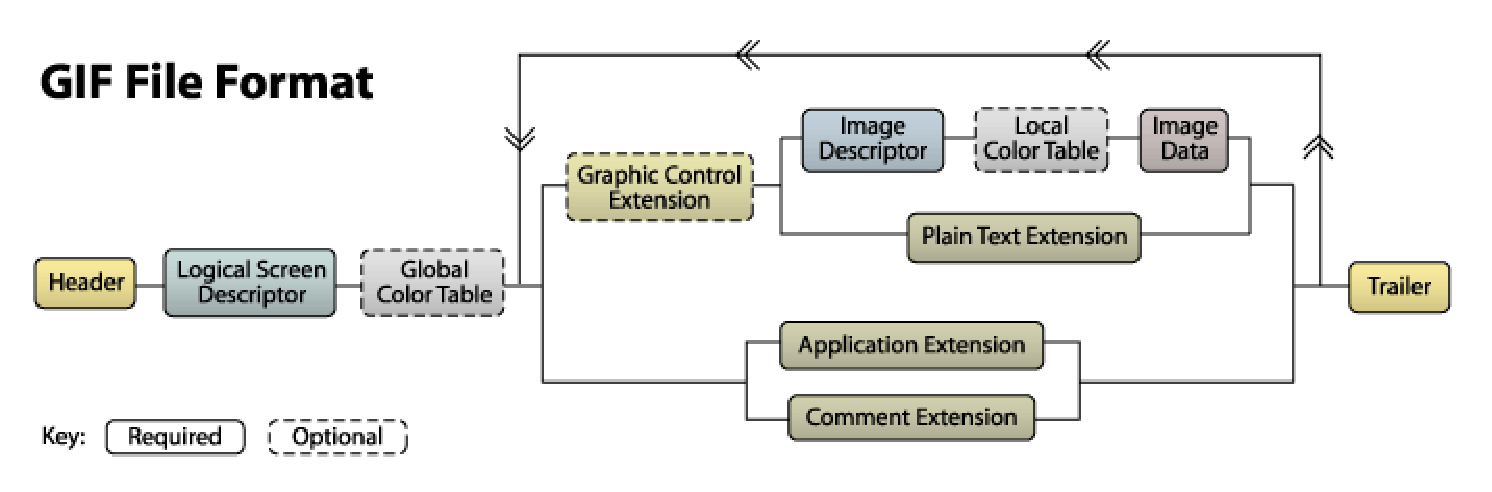
\includegraphics[width=15cm]{gif_structure.eps}


\subsection {Application du LSB}
Nous avons choisi de cacher des informations dans les couleurs qui se trouvent dans les Local Color Table. 
Cette section facultative peut revenir devant chaque bloc image data. Si cette section n'existe pas, nous la rajoutons.\\\\

Il est possible de calculer la taille maximale du message cachée à l'avance : 
en comptant le nombre de bloc image data et en le multipliant par le nombre de byte dans la Global Color Table.


\subsection {Avancement}
\subsubsection {Lecture}
Le programme peut déja lire un gif en entier, section par section. 
Les tailles des sections sont indiquées à des endroits différents par sections. 
La lecture se fait donc différemment en fonction de la section.\\\\

De plus, on peut déja savoir le nombre maximal de Local Color Table pour le fichier modifié.

\subsubsection {Lecture}
Le programme réécrit le gif dans un nouveau fichier, en insérant des Local Color Table, identique à la Global Color Table. 
Ceci permettra d'y insérer un message. 
L'insertion du message devrait être évidente, vue qu'elle sera presque identique à la stéganographie dans un fichier bitmap.\\\\

Il y a toutefois encore un bug dans la réécriture du fichier gif, probablement à l'écriture des nouvelles Local Color Table.